\section{LISA Interferometric Detection System}
\label{sec:modelling}
We now describe the LISA \ac{IDS} and present a mathematical model of the noises. We specifically focus on relevant elements for laser frequency noise and \ac{USO} jitter propagation and coupling. %Although in the real case, the clock noise suppression procedure relies on the use of the reference interferometer, here we focus on the interspacecraft interferometer as the test mass and reference interferometers are currently not included in our setup. 


\subsection{Interferometric Phase Measurements}
Each of the three identical LISA satellites carries two lasers on board. We refer to one as the local laser and the other as the adjacent laser. These two laser fields interfere on the test-mass and reference interferometers on the two optical benches of the spacecraft. In addition, the local laser interferes with the laser received from a distant spacecraft on the science interferometer. It is this science interferometer that encodes the gravitational-wave signal by measuring fluctuations in the spacecraft-to-spacecraft distance, while the test mass interferometer will measure the spacecraft-to-test mass displacement. In Figure \ref{fig:armlink} (a), a simplified LISA two-way armlink involving only the science interferometer is shown.

We begin by writing the optical phase of the laser field originating from \ac{MOSA} $ij$ on spacecraft $i$ as a function of a common modelling time $t$:
\begin{equation}\label{total_phase}
    \Phi_{ij}(t) = \nu_{ij} t + \delta \phi_{ij}(t),
\end{equation}
where $\nu_{ij}$ denotes the nominal carrier frequency and $\delta \phi_{ij}(t)$ represents the intrinsic laser phase noise. Throughout this section, phases are expressed in cycles, frequencies in Hz, and clock errors in seconds. Capital $\Phi$ denotes total phase, while $\delta\phi$ denotes phase fluctuations about the nominal linear evolution. Nominal carrier and modulation frequencies are assumed constant. Laser phase fluctuations carry two MOSA indices here, $\delta\phi_{ij}$. The one-laser-per-spacecraft testbed uses the corresponding single-index notation $\delta\phi_i$. We define the local clock reading by $t_i=t+q_i(t)$; thus $q_i$ is a timing error, while $\dot q_i$ is a fractional-frequency error. The explicit noise-coupling equations below retain terms linear in these errors and use nominal, constant beatnote coefficients. Differences between spacecraft proper times are not modelled here.


\begin{figure*}
    \centering
    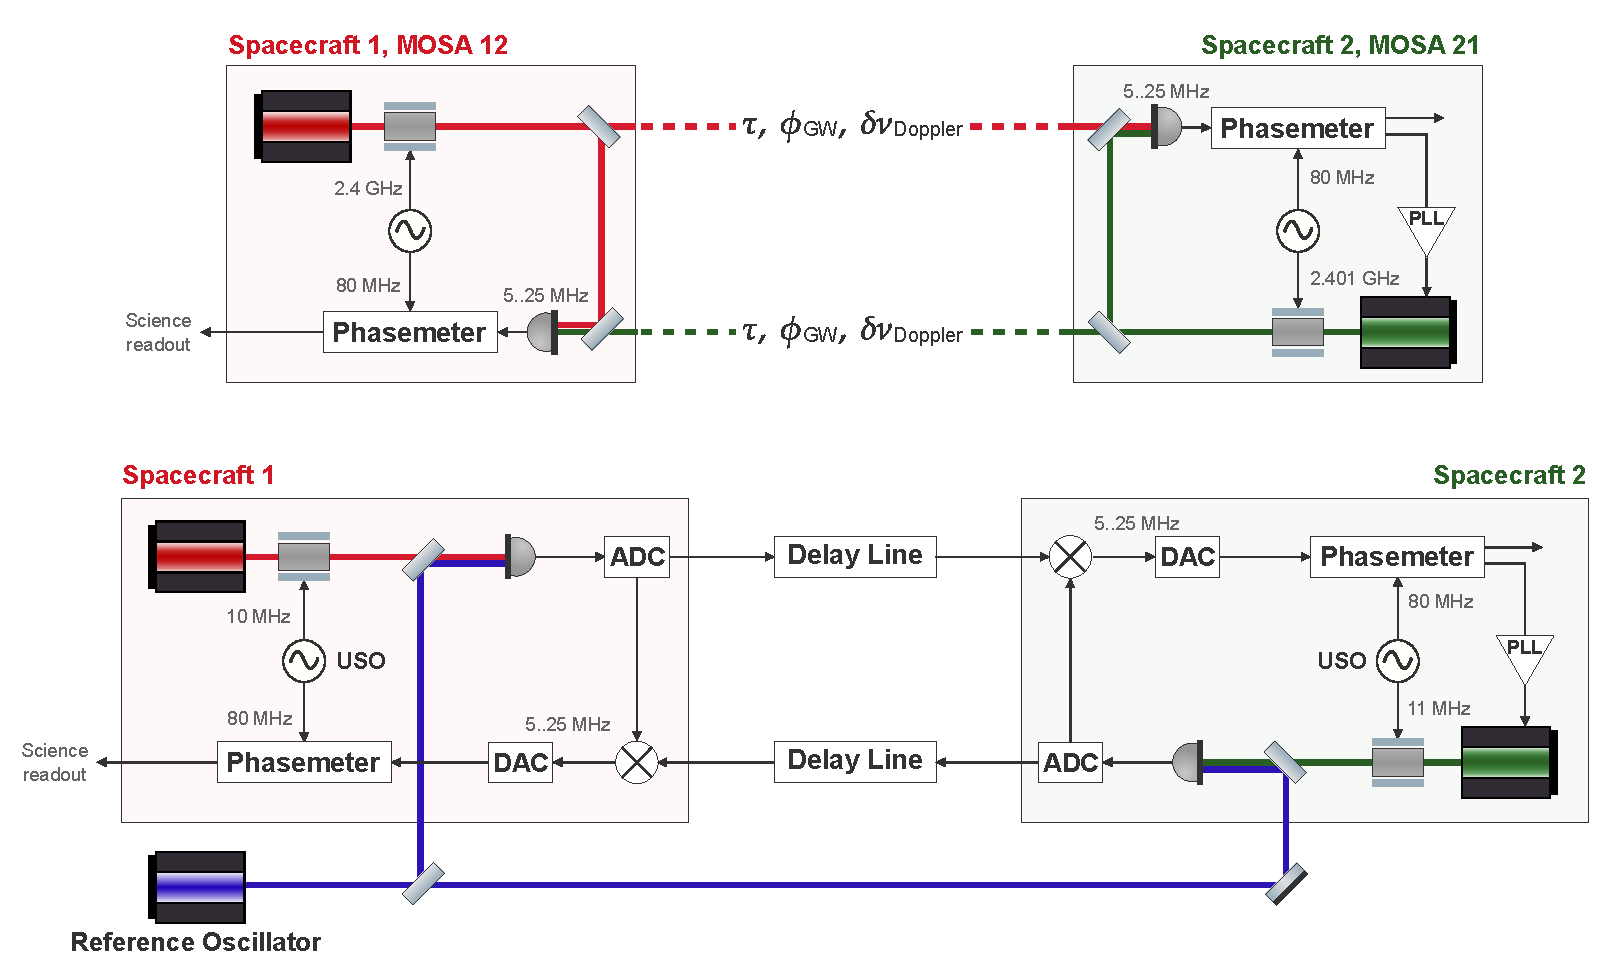
\includegraphics[width=\linewidth]{images/LISAarm-analysis.pdf}
    \caption{A comparison of the two-way links as implemented in LISA (upper) and the testbed (lower). The upper panel shows the conceptual LISA configuration: the laser on Spacecraft 1 (MOSA 12) is phase-modulated at approximately 2.4 GHz using the local USO and transmitted to Spacecraft 2 (MOSA 21). The received beam interferes with the local laser, producing heterodyne beat notes in the MHz range that contain gravitational-wave phase fluctuations, Doppler shifts due to orbital motion, and laser frequency noise. These beat notes are tracked by the phasemeter, which is clocked by the onboard 80 MHz sampling reference derived from the USO. The lower panel depicts the laboratory implementation of the same signal topology. Instead of physical light propagation over millions of kilometres, the inter-spacecraft delay is emulated electronically using digital delay lines between ADC and DAC stages. A common reference oscillator is used to downconvert the laser fields from hundreds of terahertz to tens of megahertz, which can then be sampled by the delay line \acp{ADC}. The actual LISA-like heterodyne beat notes are created in the mixers.}
    \label{fig:armlink}
\end{figure*}


Each of the laser fields is phase-modulated using an \ac{EOM} driven by the local USO. This is used to imprint sidebands on the laser field that carry the USO timing noise $q_i(t)$, with modulation phase noise $\nu^m_{ij}q_i(t)$. Since there is only one \ac{USO} per spacecraft, clock noise carries a single spacecraft index.

The modulation frequency $\nu^m_{ij}$ will be about 2.4 GHz, which is upconverted from the \ac{USO} via a \ac{PLL} synthesizer, preserving its noise with high fidelity. For the adjacent and opposing \ac{MOSA}s $ik$ and $ji$ respectively, the corresponding modulation frequency differs by 1 MHz, so 2.401 GHz, such that the sideband–sideband beat notes are offset by 1 MHz from the carrier–carrier beat note. The modulation depth $m= 0.53$ should be a fair trade-off between optical power in the carrier-carrier versus the sideband-sideband beat notes. The clock noise transfer scheme and its suppression are discussed further in the subsection \ref{clock noise}. Lower frequency offset sidebands will also be used for pseudo-random ranging and data transfer between the satellites, but are not covered here.

%
As the beam propagates from \ac{MOSA} $ij$ toward spacecraft $j$ and its \ac{MOSA} $ji$, it accumulates phase contributions from Doppler shifts due to the relative spacecraft motion and from gravitational waves integrated along the arm. Following the separation of background propagation and GW perturbations in \cite{bayle_unified_2023}, we write
\begin{equation}
    d^{\mathrm{tot}}_{ji}(t)=d_{ji}(t)+H_{ji}(t).
\end{equation}
Here $d_{ji}(t)$ is the background propagation time, which can vary slowly with the constellation breathing, and $H_{ji}(t)$ is its GW-induced perturbation. The first index denotes the receiving spacecraft and the second the emitting spacecraft. In the common-time model used here, this is a propagation-time decomposition; we do not include the transformations between spacecraft proper times contained in the proper pseudorange of \cite{bayle_unified_2023}. We define the delay operator using only the background propagation time,
\begin{equation}
    \mathbf D_{ji}x(t)=x\!\left(t-d_{ji}(t)\right).
\end{equation}
Applying the total propagation time to Eq.~\eqref{total_phase} and expanding to first order gives
\begin{align*}
    \Phi_{ij}\!\left(t-d_{ji}(t)-H_{ji}(t)\right)
    \simeq{}&\nu_{ij}\left[t-d_{ji}(t)\right]\\
    &+\mathbf D_{ji}\delta\phi_{ij}(t)
    -\nu_{ij}H_{ji}(t),
\end{align*}
where the product $H_{ji}\mathbf D_{ji}\delta\dot\phi_{ij}$ of the GW perturbation and laser-frequency noise has been neglected. We therefore introduce the GW phase contribution
\begin{equation}\label{eq:gw_phase}
    \delta\phi^{\mathrm{GW}}_{ji}(t)=-\nu_{ij}H_{ji}(t).
\end{equation}
To this order, the received total phase is $\mathbf D_{ji}\Phi_{ij}(t)+\delta\phi^{\mathrm{GW}}_{ji}(t)$: the GW signal is an additive phase contribution, separate from the background delay operator. For constant $\nu_{ij}$, the corresponding frequency fluctuation is $\delta\dot\phi^{\mathrm{GW}}_{ji}=-\nu_{ij}\dot H_{ji}$.

At spacecraft $j$, the received field $i$ interferes with the local laser field of phase $\Phi_{ji}(t)$ on a photodetector. The resulting heterodyne signal contains both the carrier–carrier beat note and the sideband–sideband beat notes. Additional cross terms lie outside the heterodyne range of the phasemeter, 5 to 25 MHz.

The electrical signal from the photodetector is then digitized by the \ac{PMS} front-end electronics. The sampling process introduces a coupling of the local USO timing error $q_j(t)$ into the measured phase. With $t_j=t+q_j(t)$ and a signed distant-minus-local beat frequency, the first-order sampling contribution is minus the beat frequency times $q_j(t)$. We define the nominal carrier coefficient
\begin{equation}
    \alpha_{ji}=\Delta\nu_{ji}=\nu_{ij}-\nu_{ji}.
\end{equation}
After subtracting the nominal phase evolution, we can write the phase fluctuations of the carrier-carrier beat note measurement
\begin{equation}\label{Main_LISA_eq}
    \begin{aligned}
    \delta\phi^{\text{c}}_{ji}(t)={}&\mathbf D_{ji}\delta\phi_{ij}(t)-\delta\phi_{ji}(t)\\
    &+\delta\phi^{\mathrm{GW}}_{ji}(t)-\alpha_{ji}q_j(t).
    \end{aligned}
\end{equation}

The signal is then passed to \acp{DPLL}, which demodulate the carrier and sideband beat notes and extract the phase fluctuations of each. So the phasemeter produces three measurements from the science interferometer photodetector that are of interest to us: the carrier beat note, which contains the gravitational-wave signal of interest, and the sideband readouts, which are used for clock jitter suppression. For all measurement readouts, we adopt the LISA convention that phases are written as “distant minus local.”\footnote{In practice, the sign depends on the frequencies constituting the beat note as the phasemeter only sees the absolute value of the difference. However, we can always get this knowledge from the frequency planning.} The carrier phase measurement recorded on spacecraft $j$ for the light received from spacecraft $i$ is
\begin{align}
    \text{sci}^{\text{c}}_{ji}(t) = & \mathbf{D}_{ji}\delta \phi_{ij}(t)-\delta \phi_{ji}(t)-\alpha_{ji}q_j(t)\nonumber\\[3pt]
    &+\delta\phi^{\mathrm{GW}}_{ji}(t)+N^{\text{c}}_{ji}(t)\nonumber\\[3pt]
    &-\frac{\nu_0}{c}\left(\mathbf{n}_{ij}\cdot \mathbf{D}_{ji}\bm{\Delta}_{ij}(t)+\mathbf{n}_{ji}\cdot\bm{\Delta}_{ji}(t)\right),
\end{align}
The term $N^{\mathrm{c}}_{ji}(t)$ represents combined readout noise from optical path-length fluctuations and electronics. The vectors $\bm{\Delta}_{ij}(t)$ are optical-bench displacements in metres. The unit vector $\mathbf n_{ji}$ points along the incoming beam from spacecraft $i$ to spacecraft $j$, and $\mathbf n_{ij}=-\mathbf n_{ji}$ in the geometry used for these displacement terms. We use a common nominal optical frequency $\nu_0$ in all displacement couplings, neglecting relative optical-frequency offsets there; the distinct frequencies are retained in the heterodyne clock coefficients. Thus $\nu_0/c$ converts a one-way displacement into phase in cycles.

%\Delta\omega^{\mathrm{sb}}_{ij}t+ 
The corresponding upper sideband–sideband beat note readout can be written as
\begin{align}\label{SB_meas}
    \text{sci}^{\mathrm{sb,+}}_{ji}(t)=&
    \mathbf{D}_{ji}\delta\phi_{ij}(t)- \delta\phi_{ji}(t)- \gamma_{ji}\, q_j(t)\nonumber\\[3pt]
    &+\delta\phi^{\mathrm{GW}}_{ji}(t)+N^{\mathrm{sb,+}}_{ji}(t)\nonumber\\[3pt]
    &-\frac{\nu_0}{c}\left(\mathbf{n}_{ij}\cdot \mathbf{D}_{ji}\bm{\Delta}_{ij}(t)+\mathbf{n}_{ji}\cdot\bm{\Delta}_{ji}(t)\right)
    \nonumber\\[3pt]
    &+\nu^m_{ij} \mathbf{D}_{ji} q_i(t)- \nu^m_{ji} q_j(t).
\end{align}
The sideband clock coupling coefficient is
\begin{equation}
    \gamma_{ji} =\Delta\nu_{ji}+\nu^m_{ij}-\nu^m_{ji}=\Delta\nu_{ji}+\Delta\nu^m_{ji}= \Delta\nu_{ji}^{\mathrm{sb,+}}.
\end{equation}
Again, the term $N^{\mathrm{sb,+}}_{ji}(t)$ represents stochastic readout noise specific to the upper sideband measurement. The lower sideband has the same laser phase noise but the opposite sign for each modulation contribution, including the modulation part of the beatnote coefficient. We show the upper sideband explicitly. Relative corrections of order $\nu^m/\nu_0$ to the displacement coupling are neglected. We also neglect the relative correction $\nu^m_{ij}/\nu_{ij}$ to the GW coupling: the exact upper-sideband contribution at this order is $-(\nu_{ij}+\nu^m_{ij})H_{ji}$, approximated here by the same $\delta\phi^{\mathrm{GW}}_{ji}$ as in the carrier. This makes the retained GW term common to the carrier and both sidebands. 

For completeness, we also write out the reference and test mass interferometer readings on \ac{MOSA} $ji$
\begin{align}
\text{tm}_{ji}(t)= &
\delta\phi_{jk}(t)-\delta\phi_{ji}(t)
+\beta_{ji}q_j(t)+\mu_{j}(t)+N^{\text{tm}}_{ji}(t)\nonumber\\[3pt]
&+\frac{2\nu_0}{c}
\mathbf{n}_{ji}\cdot\left(\bm{\delta}_{ji}(t)-\bm{\Delta}_{ji}(t)\right),\\[5pt]
\text{ref}_{ji}(t)&=\delta\phi_{jk}(t)-\delta\phi_{ji}(t)+\beta_{ji}q_j(t)+\mu_{j}(t)+N^{\text{ref}}_{ji}(t).
\end{align}
Here we have introduced the fiber noise $\mu_{j}$ coming from the optical fiber that exchanges the local and adjacent laser fields between \ac{MOSA} $ji$ and \ac{MOSA} $jk$ . This term is typically referred to as the backlink noise. We have assumed it to be independent of the direction of propagation of the optical beams within. The vector $\bm{\delta}_{ji}$ is the test-mass displacement in metres, including displacement produced by acceleration noise; it is not itself an acceleration. With the same sampling convention, the reference and test-mass clock coefficient is
\begin{equation}
    \beta_{ji}=\nu_{ji}-\nu_{jk}.
\end{equation}
It has the opposite sign to the adjacent-minus-local beat frequency, which explains the plus sign multiplying $\beta_{ji}q_j$ in the readouts.

In reality, the beat notes will contain many more noise sources, for example, the tilt-to-length coupling or \ac{ADC} noise. Since our testbed does not include the test mass or reference interferometers, the associated optical-bench motion, backlink fiber noise, and test mass acceleration noise terms will not be considered in the following sections.


\subsection{Laser Noise and \ac{TDI}}

In the LISA measurement system, laser frequency noise is first reduced onboard by locking one laser to an optical resonator and phase-locking the remaining lasers to this pre-stabilized reference with fixed frequency offsets. The last step ensures that all heterodyne beat notes remain within the phasemeter bandwidth while maintaining coherent phase relationships between spacecraft. However, residual laser frequency noise remains many orders of magnitude above the displacement sensitivity requirement and must be suppressed in post-processing. \ac{TDI} achieves this by forming linear combinations of one-way phase measurements and appropriately delayed copies thereof, effectively synthesizing an equal-arm interferometer in post-processing.

Because the inter-spacecraft separations vary in time due to orbital motion, the light-travel times entering the delay operators are time-dependent. As a result, delay operators do not commute, and first-generation \ac{TDI} combinations do not yield exact cancellation. Second-generation \ac{TDI} combinations account for time-varying delays and achieve exact cancellation for delays that are approximately linear in time.

Accurate knowledge of the delays is essential, as an error $\delta d$ in the applied delay leads to residual laser noise proportional to the time derivative of the laser phase noise. This sets the requirement on delay knowledge to approximately one meter, motivating LISA’s dedicated ranging system.

Before \ac{TDI} is implemented, intermediary variables are constructed. The reference and test-mass interferometer readings remove optical-bench displacement noise, as discussed in \cite{otto2012tdi,tinto2018time}. To make the signs explicit, define
\begin{align*}
    T_{ji}&=\text{tm}_{ji}-\text{ref}_{ji},\\
    \xi_{ji}&=\text{sci}^{\mathrm c}_{ji}
    -\frac12\left(T_{ji}+\mathbf D_{ji}T_{ij}\right).
\end{align*}
Within the common-optical-frequency approximation above, the bench terms cancel, leaving the test-mass contribution
\begin{equation*}
    M_{ji}=-\frac{\nu_0}{c}\left[
    \mathbf n_{ji}\cdot\bm\delta_{ji}(t)
    +\mathbf D_{ji}\!\left(\mathbf n_{ij}\cdot\bm\delta_{ij}(t)\right)
    \right].
\end{equation*}
The following equations omit readout noises. Reciprocal backlink noise cancels in the local reference difference
\begin{equation*}
    z_{ji}=\frac12\left(\text{ref}_{ji}-\text{ref}_{jk}\right)
    =\delta\phi_{jk}-\delta\phi_{ji}+\beta_{ji}q_j.
\end{equation*}
For cyclic triples $(i,j,k)=(1,2,3),(2,3,1),(3,1,2)$, the intermediate variables can then be defined as
\begin{align*}
    \eta_{ji}&=\xi_{ji}-z_{ji}\\
    &=\mathbf D_{ji}\delta\phi_{ij}(t)-\delta\phi_{jk}(t)
    -(\alpha_{ji}+\beta_{ji})q_j(t)\\
    &\quad+\delta\phi^{\mathrm{GW}}_{ji}(t)+M_{ji}(t),\\[3pt]
    \eta_{ij}&=\xi_{ij}+\mathbf D_{ij}z_{ji}\\
    &=\mathbf D_{ij}\delta\phi_{jk}(t)-\delta\phi_{ij}(t)
    -\alpha_{ij}q_i(t)\\
    &\quad+\mathbf D_{ij}\!\left[\beta_{ji}q_j(t)\right]\\
    &\quad+\delta\phi^{\mathrm{GW}}_{ij}(t)+M_{ij}(t).
\end{align*}
Here $M_{ij}$ is obtained by exchanging $i$ and $j$ in $M_{ji}$. These combinations reduce the number of independent laser phase noises from six to three, retaining $\delta\phi_{12}$, $\delta\phi_{23}$ and $\delta\phi_{31}$, while removing the optical-bench displacement terms. The construction introduces an asymmetry between the two link orientations.

Further, as an example, a commonly used first-generation Michelson-type \ac{TDI} observable synthesised at spacecraft $i$ is the $X_i$ combination, which can be written as
\begin{align}
X_i(t) ={}&
\Bigl[(\eta_{ik}(t) + \mathcal{D}_{ik}\eta_{ki}(t))+
\mathcal{D}_{ik}\mathcal{D}_{ki}(\eta_{ij}(t) + \mathcal{D}_{ij}\eta_{ji}(t))
\Bigr]\nonumber\\[3pt]
&-\Bigl[(\eta_{ij}(t) + \mathcal{D}_{ij}\eta_{ji}(t))+
\mathcal{D}_{ij}\mathcal{D}_{ji}(\eta_{ik}(t) + \mathcal{D}_{ik}\eta_{ki}(t))
\Bigr],
\end{align}

where $\mathcal{D}_{ij}$ is the delay operator -- the cursive indicates it is being applied in post-processing. 


%\begin{align*}
%    X_2(t)=[\mathcal{D}_{ij}\mathcal{D}_{ji}\mathcal{D}_{ik}\mathcal{D}_{ki}-1][(\eta_{ik}+\mathcal{D}_{ik}\eta_{ki})+\mathcal{D}_{ik}\mathcal{D}_{ki}(\eta_{ij}+\mathcal{D}_{ij}\eta_{ji})]\\
%    -[\mathcal{D}_{ik}\mathcal{D}_{ki}\mathcal{D}_{ij}\mathcal{D}_{ji}-1][(\eta_{ij}+\mathcal{D}_{ij}\eta_{ji})+\mathcal{D}_{ij}\mathcal{D}_{ij}(\eta_{ik}+\mathcal{D}_{ik}\eta_{ki})].
%\end{align*}



\subsection{Clock-noise Coupling and Correction}
\label{clock noise}
The second-largest noise contribution in the raw measurements is timing jitter arising from the USOs [red book]. Similarly to laser frequency noise, it exceeds the sensitivity requirement by several orders of magnitude and must be removed in post-processing before gravitational wave signals can be recovered. Unlike laser frequency noise, it couples into the measurement only locally at one spacecraft. Hence, to still allow for a similar differential measurement of the clock noise, the laser fields exchanged between the satellites are modulated with a signal derived from the \acp{USO}. From the upper and lower sideband phase measurements at the science interferometer, as written in (\ref{SB_meas}), a correcting term can be constructed. \\
Using the phase-domain counterpart of the clock-transfer construction in \cite{hartwig_clock-jitter_2021}, and neglecting readout and modulation noises initially, we define
\begin{equation}\label{correction variables}
    r_{ji} = \frac{\text{sci}^{\mathrm{sb,+}}_{ji}(t)- \text{sci}^{\mathrm{c}}_{ji}(t)}{\nu^m_{ij}}=\mathbf{D}_{ji}q_i(t)-q_j(t).
\end{equation}
The common GW phase cancels in this difference under the sideband GW-coupling approximation stated above. The normalization uses the transmitted modulation frequency $\nu^m_{ij}$, so these phase-domain $r_{ji}$ have units of seconds. Equivalently, using both sidebands gives $r_{ji}=(\text{sci}^{\mathrm{sb,+}}_{ji}-\text{sci}^{\mathrm{sb,-}}_{ji})/(2\nu^m_{ij})$ in the same noise-free approximation. As can be seen, the $r$ variables contain the USO noise in the same form as the overall intersatellite interferometer readouts contain laser frequency noise. Hence, as shown in \cite{hartwig_clock-jitter_2021}, these variables can be used to build up correcting terms using Vallisneri's algorithm.\\
For clock noise removal to work properly, the modulation must track the effective measurement-clock reference. Let $N_{ij}(t)$ denote differential timing noise in the tone derivation for MOSA $ij$, in seconds, and let $N^m_{ij}(t)$ denote additional optical modulation phase noise, in cycles. The excess upper-sideband phase is
\begin{equation*}
    m_{ij}(t)=\nu^m_{ij}N_{ij}(t)+N^m_{ij}(t).
\end{equation*}
Including these terms and readout noise gives
\begin{align*}
    r_{ji}={}&\mathbf D_{ji}q_i-q_j
    +\frac{\mathbf D_{ji}m_{ij}-m_{ji}}{\nu^m_{ij}}\\
    &+\frac{N^{\mathrm{sb,+}}_{ji}-N^{\mathrm c}_{ji}}{\nu^m_{ij}}.
\end{align*}
In particular, the local tone-derivation noise enters with the factor $-\nu^m_{ji}/\nu^m_{ij}$; it cannot be assigned unit weight when the modulation frequencies differ. These excess noises propagate through the clock correction into the corrected measurements.\\
The distinction between timing and direct phase noise also matters for the modulation-frequency choice. Referred to the source modulation frequency, $m_{ij}/\nu^m_{ij}=N_{ij}+N^m_{ij}/\nu^m_{ij}$. Increasing the transmitted and local modulation frequencies by the same factor therefore suppresses a fixed direct phase-noise contribution to $r_{ji}$, but not a fixed differential timing noise; the local timing term retains the ratio $\nu^m_{ji}/\nu^m_{ij}$. A measurement of the combined modulation noise at a single frequency does not by itself separate these contributions. This limitation applies to both LISA and the testbed, and the scaling is conditional on the underlying noises remaining unchanged when the modulation frequency is increased.

The ultimate clock reference will be the pilot tone, which is also derived from the \ac{USO} and is used to correct \ac{ADC} sampling jitter within the \ac{PMS}. The differential timing jitter between the modulating frequency of 2.4 GHz and the corresponding pilot tone will be below 50 fs/$\sqrt{\text{Hz}}$ as per requirements. For the adjacent 2.401 GHz, this requirement is relaxed as the digital synthesis from the 10 MHz \ac{USO} can not be as noise-free. This additional noise is called 'modulation noise' in \cite{hartwig_clock-jitter_2021}. Hence, the corresponding clock noise correcting $ r$-variables themselves need correcting. For this purpose, LISA reference interferometers also measure an onboard sideband-sideband beat note. From these, similar correcting variables as (\ref{correction variables}) are defined and can be used to remove the accessible differential modulation-noise contribution; modulation noise is not eliminated completely.

\begin{figure}
    \centering
    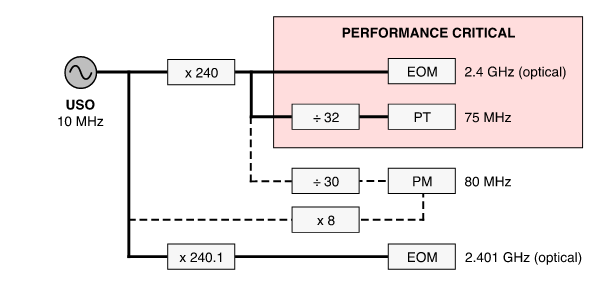
\includegraphics[width=\linewidth]{images/FDM.png}
    \caption{Clock-generation and distribution scheme highlighting performance-critical paths. A 10 MHz USO signal is multiplied to 2.4 GHz for optical sideband modulation via the \ac{EOM}, forming the primary clock-transfer tone. Parallel synthesis chains generate the 75 MHz \ac{PT} used for ADC timing correction and the 80 MHz sampling clock driving the \ac{PM}. The shaded region marks the performance-critical elements, where clock phase noise must be preserved with high fidelity. A slightly offset 2.401 GHz modulation is generated for the opposite spacecraft to produce MHz-offset sideband–sideband beat notes. The architecture ensures coherent distribution of clock noise into both optical modulation and digital sampling paths, enabling subsequent clock-noise suppression in post-processing. }
    \label{fig:fdm}
\end{figure}

%For the clock jitter terms, we can generally assume that the delay operators commute.
\begin{figure}
    \centering
    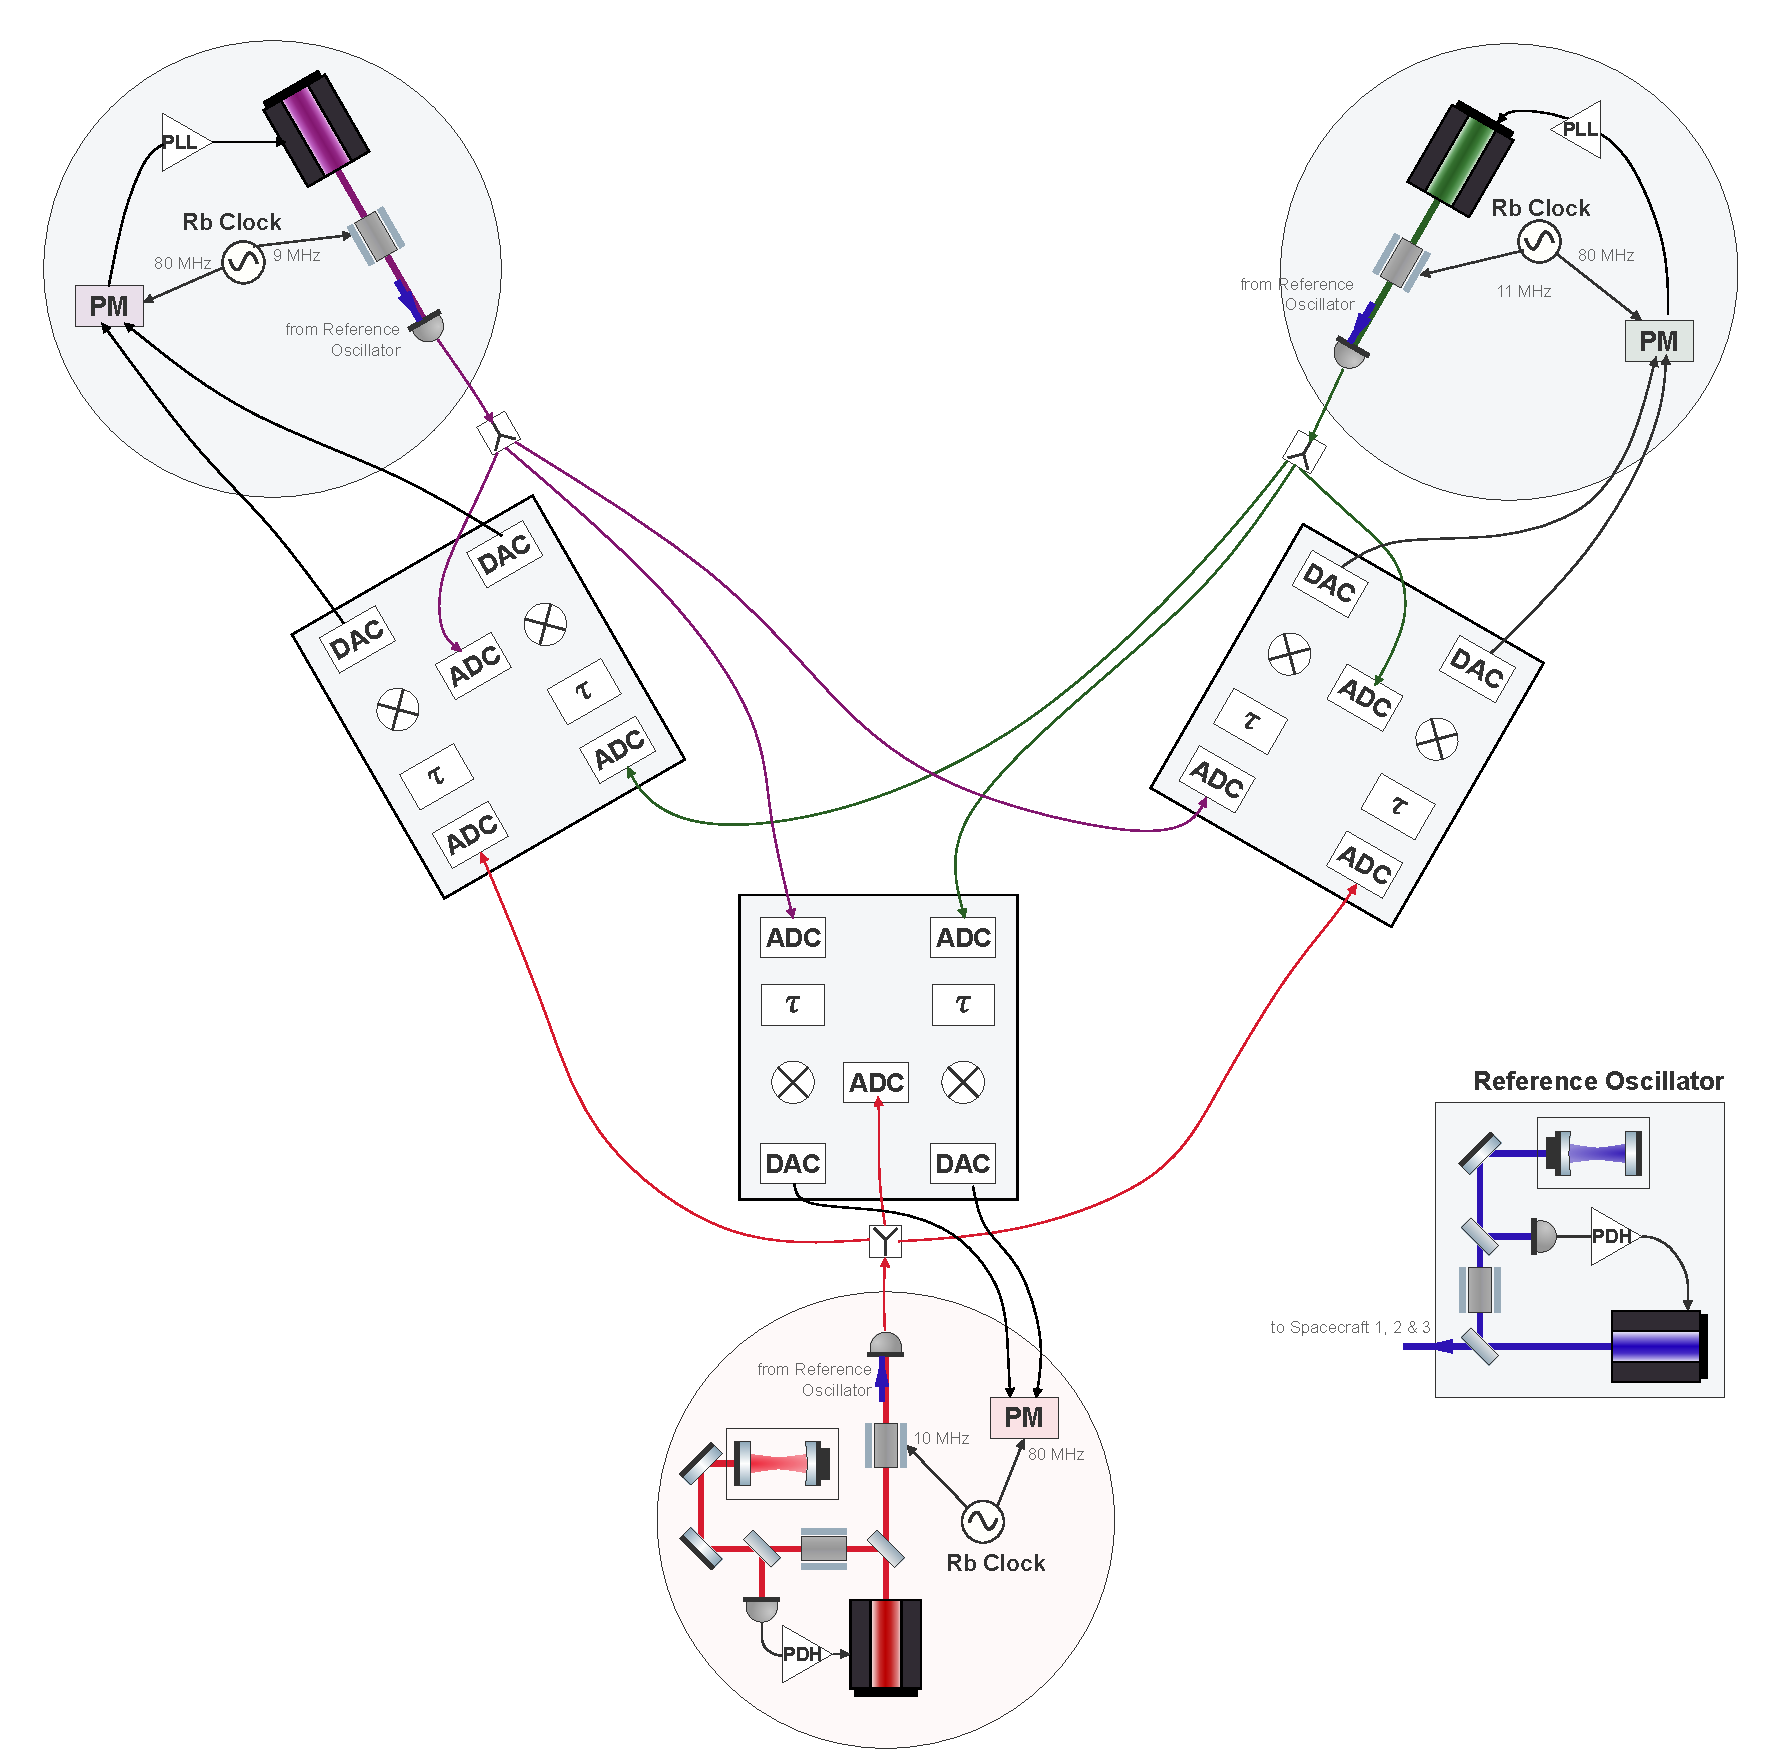
\includegraphics[width=\linewidth]{images/3arm.pdf}
    \caption{Triangular LISA testbed laboratory implementation. Three simulated spacecraft are arranged in a closed topology, each equipped with a laser, phasemeter (PM), and an independent Rb clock. The MHz heterodyne beat notes are digitised and routed through programmable delay blocks that emulate the inter-spacecraft light-travel times required for \ac{TDI}. In general, two signals are delayed on each delay-line board; these are configured to represent the incoming links to a given spacecraft, while the clock driving that delay board is matched to the corresponding spacecraft phasemeter. A common optical reference oscillator provides pre-stabilisation via PDH locking. This architecture preserves the essential structure of LISA’s one-way measurements while replacing physical arm lengths with electronic delays.}
    \label{fig:triangular}
\end{figure}
%Due to the differences in how the modulating signal vs the pilot tone on the left and right side MOSAs are derived, the correcting terms for the right side are noisier and need further corrections using the reference interferometer sideband measurements. However, as our testbed essentially implements one MOSA per spacecraft, this correction to the correcting variables can't be tested without additional hardware.